\section*{TCP: WireShark}
The connection setup packets are shown in Figure~\ref{fig:tcp1}. We can see that the connection sequence begins with the 3-way handshake. The source/receiving computer sends a SYN packet to the \texttt{compeng4dn4.mooo.com} server, with a source port of 25078, destination port of 50008, window size of 64240 bytes, and max segment size of 1460 bytes. The length is 0 as this is a SYN packet so no data is transmitted in this stage. The server responds to the source computer with a packet with the SYN and ACK bits set, with the same windows and max segment sizes. Finally, the receiving computer sends an ACK packet back to the server with the sequence number incremented by 1. The sequence number is incremented by 1 as the length of the packet was 0.

Once the handshake is completed successfully, we can see that the data transfer starts after the GET request packet. The server acknowledges this and starts sending the image data in another packet of length 1460 bytes. It then sends another packet of the same length with the PUSH flag set, which signals to the receiving computer that it must not wait for more data from the sending TCP device before passing the data to the receiving process. There is a coupling between the push function and the use of buffers of data that cross the TCP/user interface. Each time a PUSH flag is associated with data placed into the receiving user's buffer, the buffer is returned to the user for processing even if the buffer is not filled. If data arrives that fills the user's buffer before a PUSH is seen, the data is passed to the user in buffer size units.

This acknowledgement and data transfer sequence continues in packets 171, 172, 176, 177, 181, 182, 186, 187, 191, 192, 196, 197, 201, 202, 207, 208, 212, 213, 214, 218, 222, 223, 227, 228, 232, 233, and 237 until the server returns an HTTP 200 OK code in 237, which signals that the GET request has been completed successfully. Each time a data packet is transmitted by the server, the sequence number of the server packet increases by the length of the previous packet. For example, from packet 212 to 213, the sequence number increased from 23361 to 23361 + 1460 = 24821. When the receiving computer receives this packet, it responds with a packet that contains the SEQ number of the requested ACK value, and it sets its own ACK value to the previous packet SEQ number + the length of the previous packet. For example, from packet 214 to 215, the sequence number went from 26281 to 560, which is what the server requested as the ACK, and the ACK went from 560 to 26281 + 1460 = 27741. This is shown in Figure~\ref{fig:tcp2}. The server then sends a FIN-ACK packet, which means that it received the previous packet and wants to close the connection. We do not see the source computer send a FIN-ACK back because that only happens when you close the browser tab with the image.

The image that was downloaded from the server was \texttt{351.jpeg} and can be seen in Figure~\ref{fig:mooo}.
\clearpage

\begin{figure}[p]
    \centering
    \caption[tcp1]{WireShark Packet Capture 1st Half}\label{fig:tcp1}
    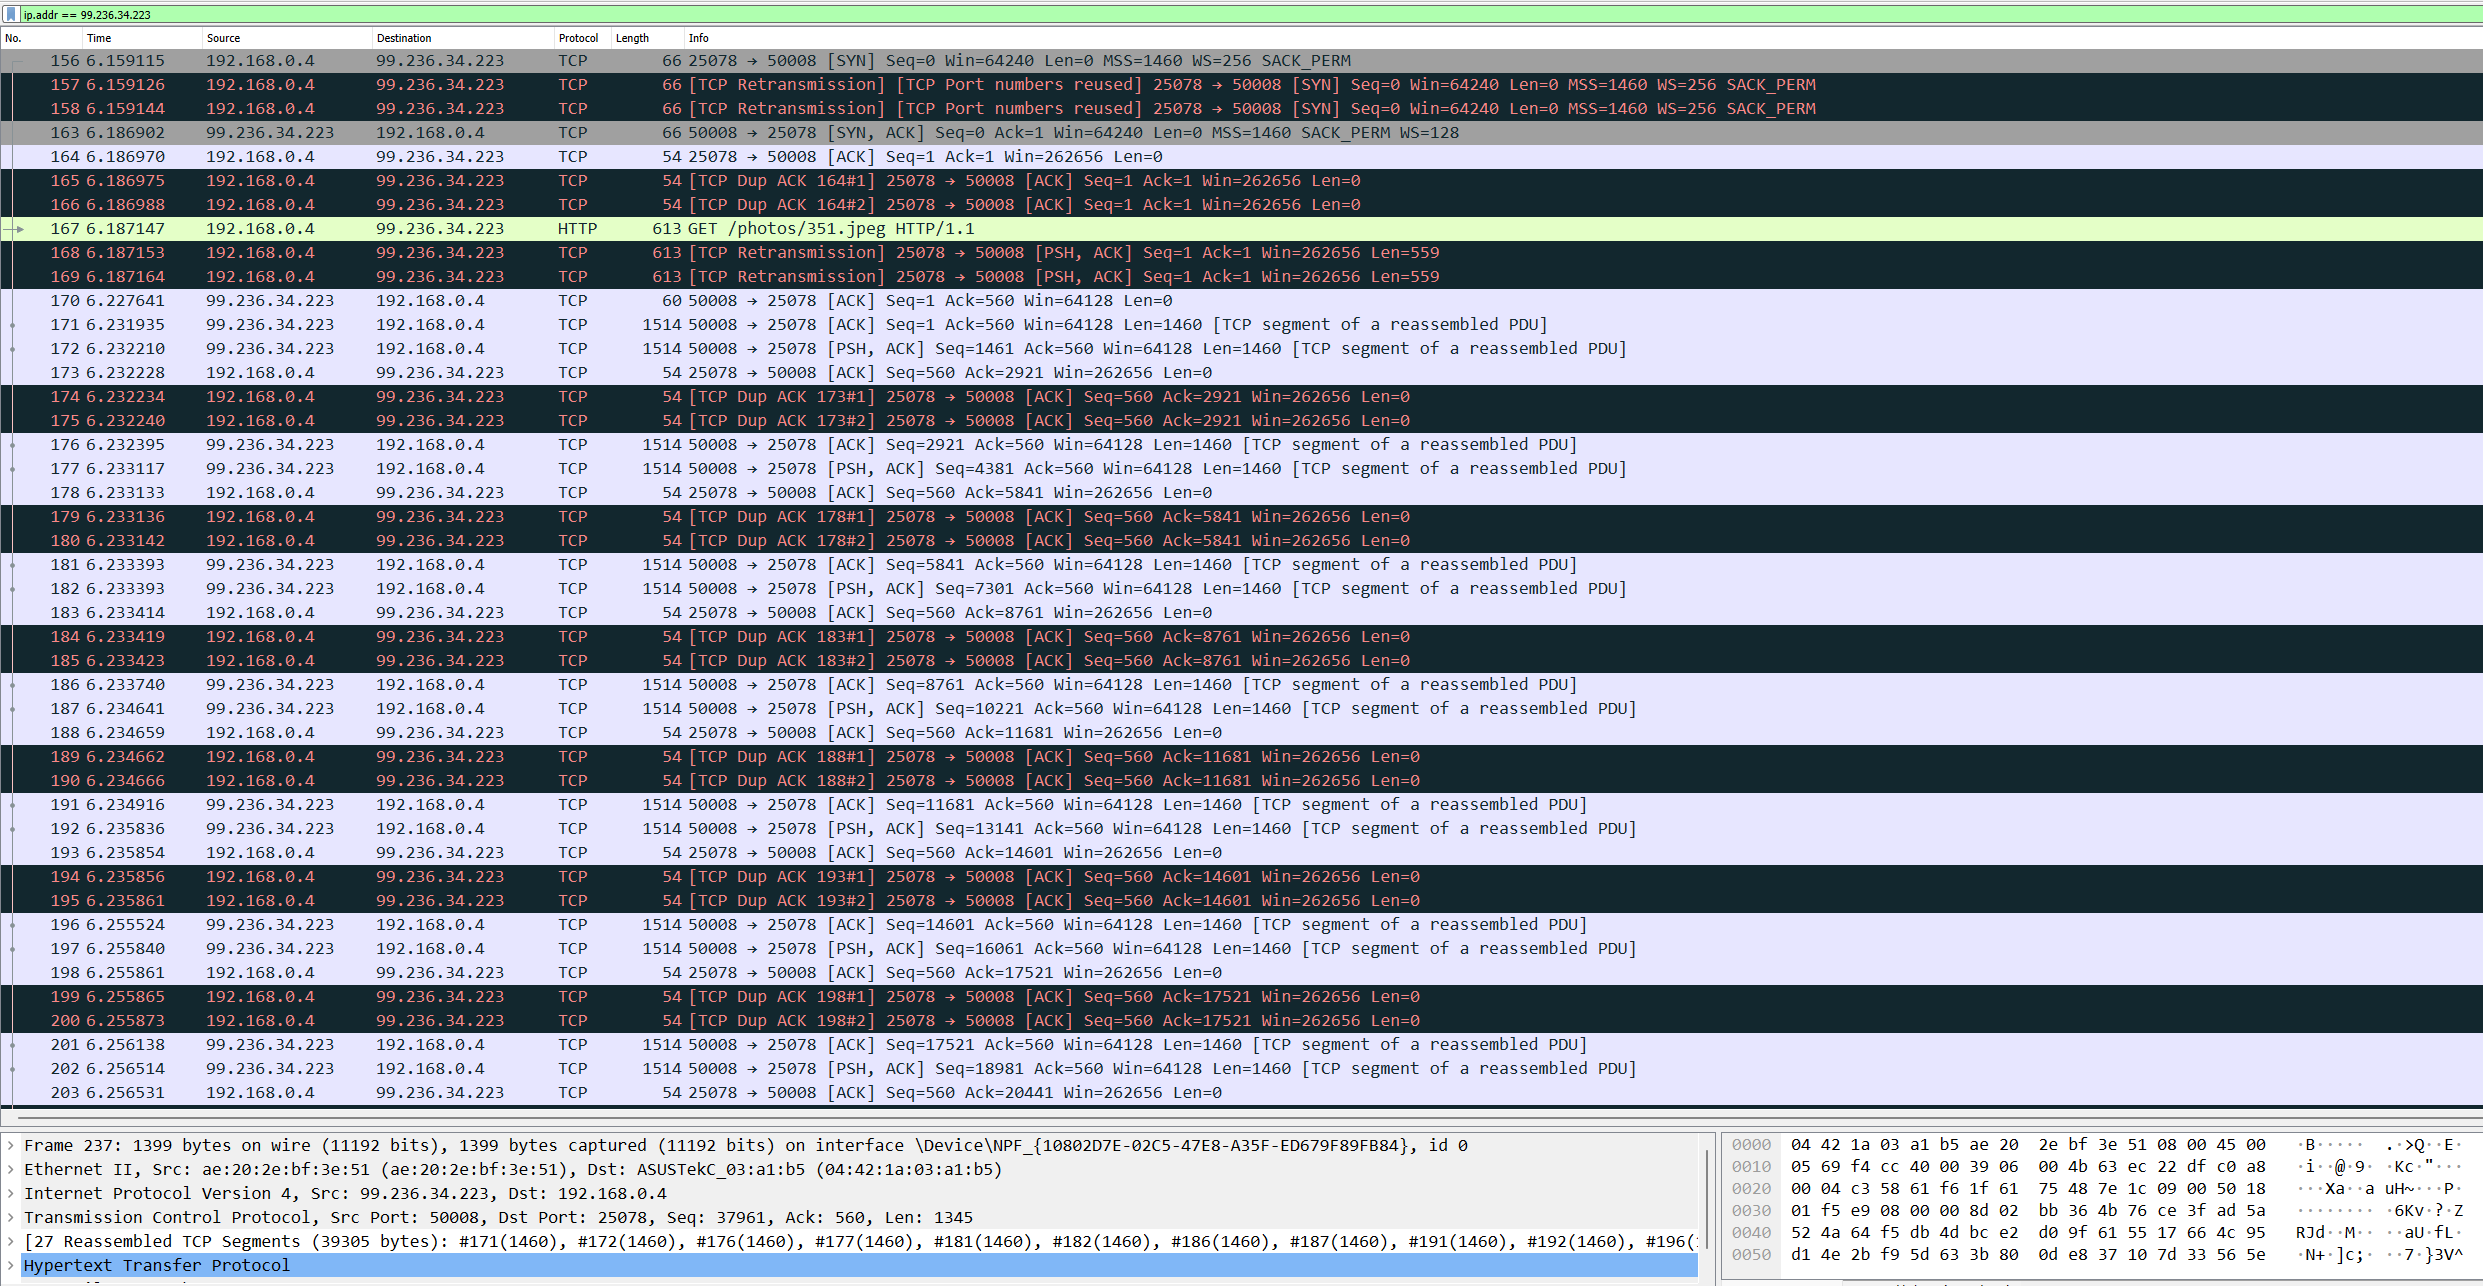
\includegraphics[width=\textwidth]{tcp_wireshark_1.png}
\end{figure}

\begin{figure}[p]
    \centering
    \caption[tcp2]{WireShark Packet Capture 2nd Half}\label{fig:tcp2}
    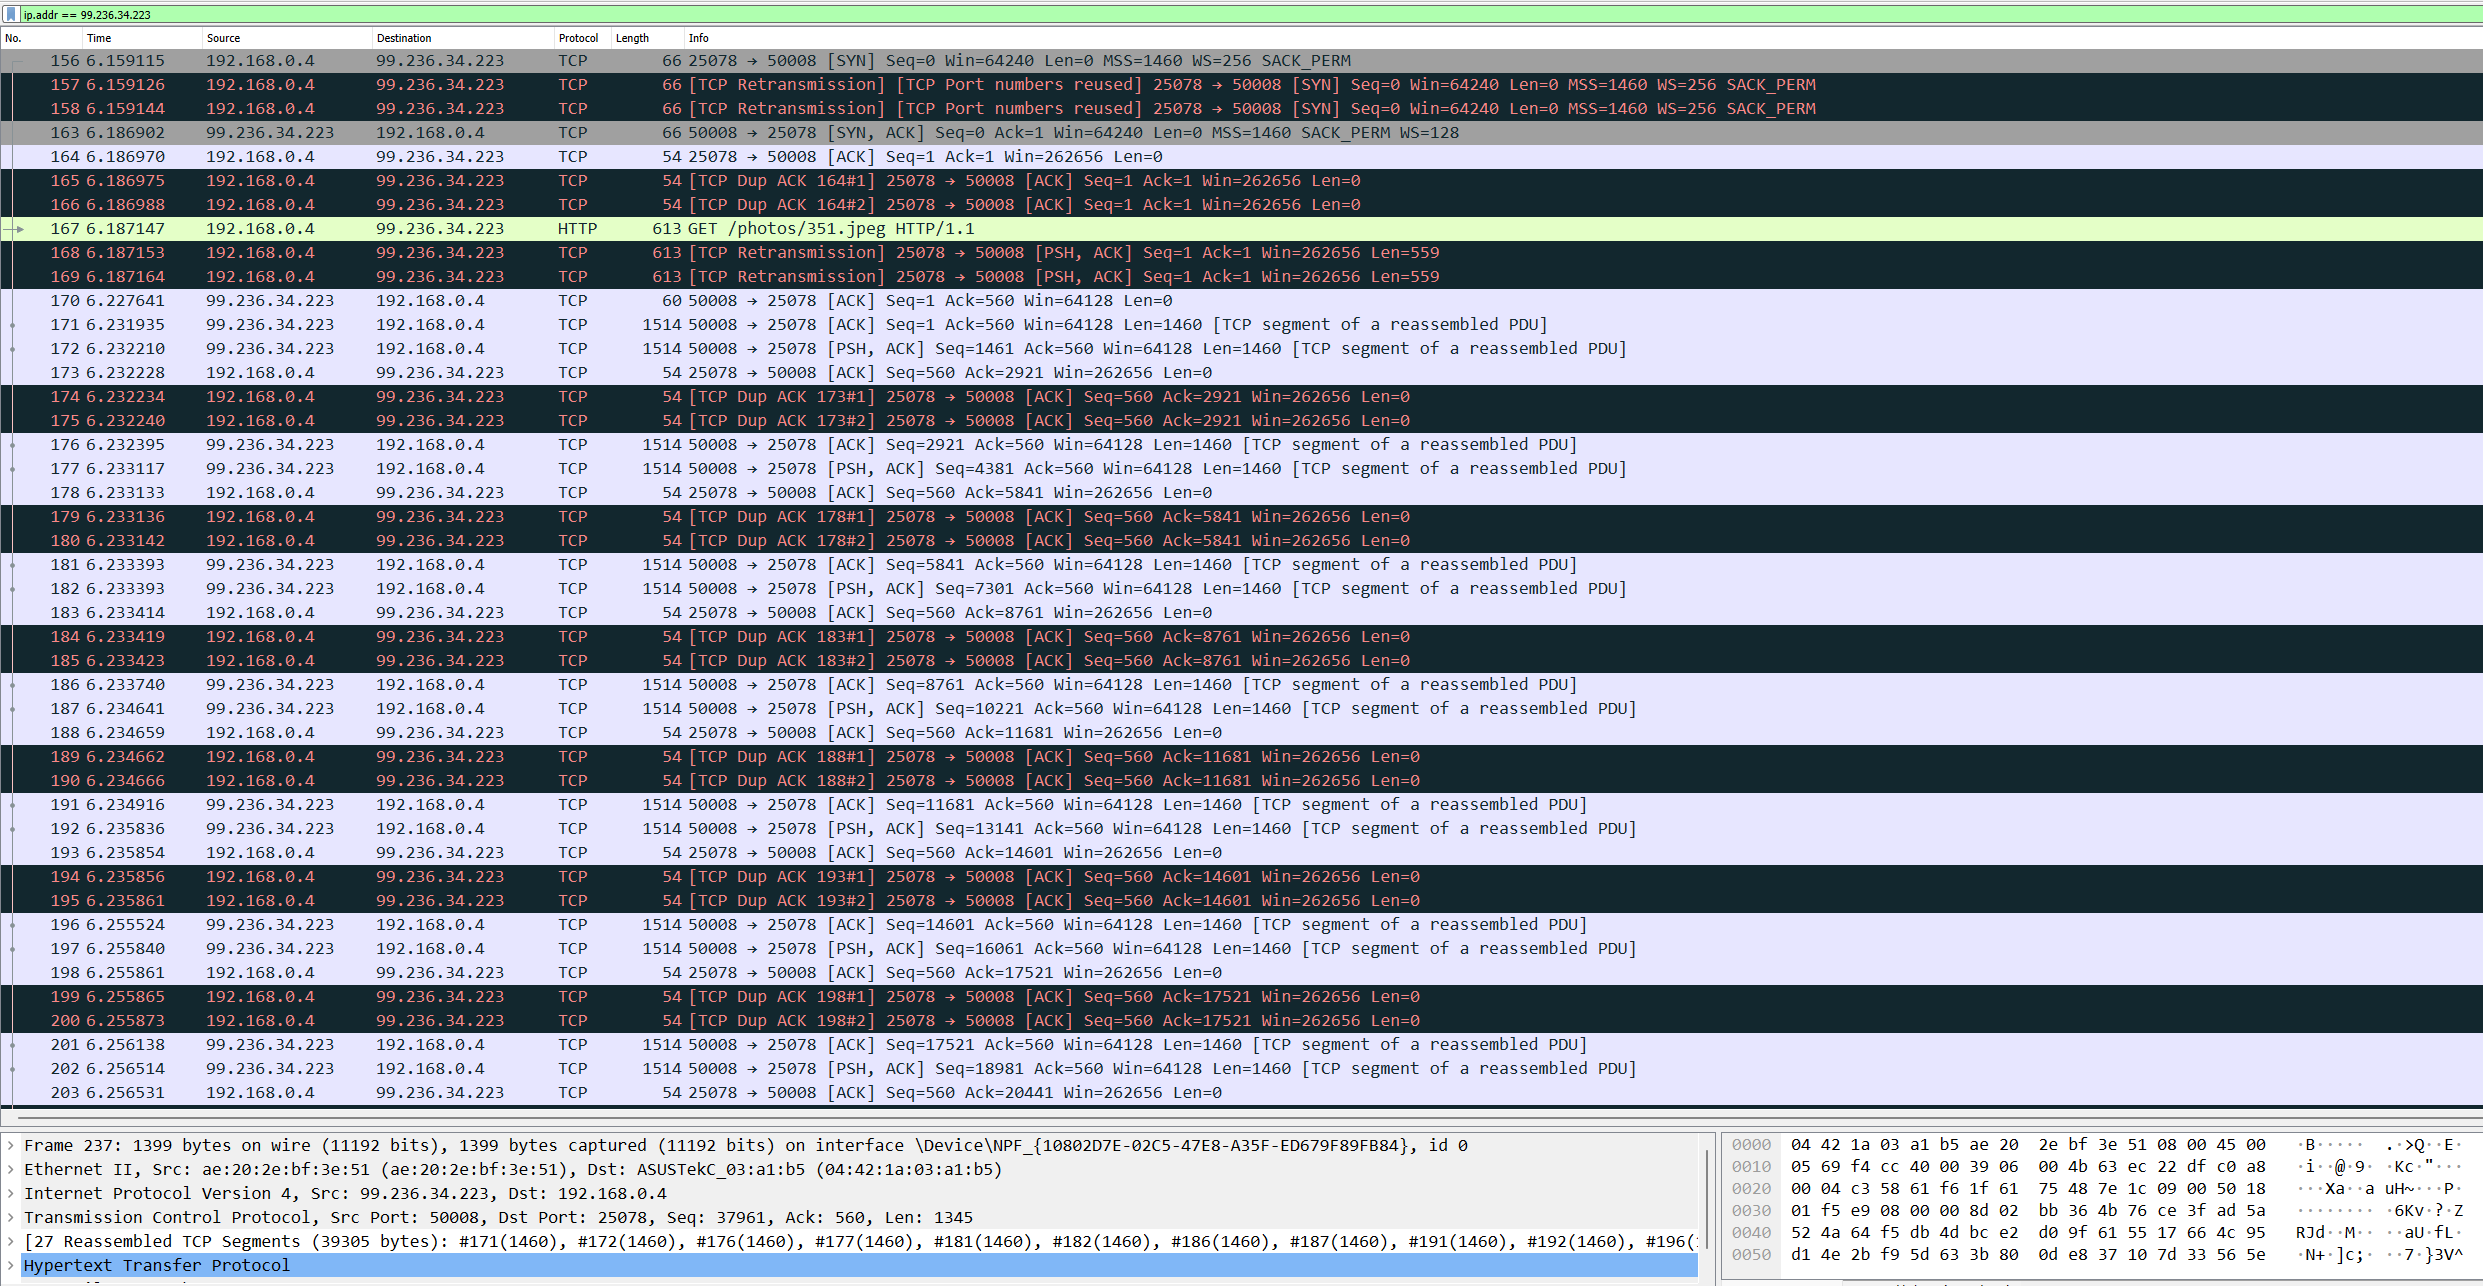
\includegraphics[width=\textwidth]{tcp_wireshark_1.png}
\end{figure}

\clearpage

\begin{figure}[htp]
    \centering
    \caption[mooo]{\url{http://compeng4dn4.mooo.com:50008/photos/351.jpeg}}\label{fig:mooo}
    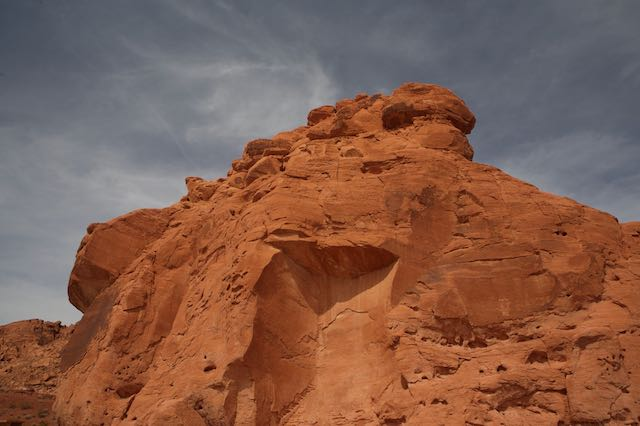
\includegraphics[width=\textwidth]{351.jpeg}
\end{figure}
